% Koma class
\documentclass[a4paper, oneside]{scrartcl}   

\usepackage{a4wide}

%------------------
% language = english
\usepackage[english, german]{babel}	% Umlaute mit \"u
\usepackage[latin1]{inputenc}
\usepackage{enumitem}

% margins + Kopf- und Fu�zeilen
\usepackage[left = 2.5cm, right = 2.5cm, top = 2cm, bottom = 3cm]{geometry}
\usepackage{scrpage2} 
\pagestyle{scrheadings}
\clearscrheadfoot
\rehead{\headmark}
\lehead{\pagemark}
\lohead{\headmark}
\rohead{\pagemark} 

% math
\usepackage{amssymb}
\usepackage{amsmath}

% figures
\usepackage{tikz}
\usepackage{graphicx}

% section-Zaehler wird neu gesetzt:
\setcounter{section}{8}
%------------------
\author{Sascha Meiers, Martin Seeger}
\title{Exercise 8, Discrete Mathematics for Bioinformatics}
\date{Winter term 2011/2012}


\begin{document}
\maketitle

%---------------------------------------------------------------------------------------------------

\subsection{Linear Optimization}

\begin{equation}
2x_1+3x_2 = \min \Leftrightarrow -2x_1-3x_2 = \max .
\end{equation}
\begin{equation}\label{1}
3x_1+6x_2\leq 7 \Leftrightarrow 3x_1+6x_2+x_3=7,\ x_3\geq 0.
\end{equation}
\[
x_1\  \mathrm{free} \Leftrightarrow x_1 = x_4-x_5,\ x_4\geq 0,\ x_5\geq 0.
\]
Insert the previous equation into \eqref{1}:
\[
6x_2+x_3+3x_4-3x_5=7,\ x_3\geq 0,\ x_4\geq 0,\ x_5\geq 0.
\]
Finally,
\[
2x_1 + 2x_2 = 5 \Leftrightarrow 2x_2 + 2x_4 - 2x_5= 5, 
\]
\[
-2x_1-3x_2 = -3x_2-2x_4+2x_5 = \max .
\]
Summarizing,
\[
\max \left\{(-3,0,-2,2) 
\left(
 \begin{smallmatrix}
  x_2\\x_3\\x_4\\x_5
 \end{smallmatrix}
\right)
\middle| 
\begin{pmatrix}
 6 & 1 & 3 & -3\\
 2 & 0 & 2 & -2
\end{pmatrix}
\left(
 \begin{smallmatrix}
  x_2\\x_3\\x_4\\x_5
 \end{smallmatrix}\right) =
 \begin{pmatrix}
  7\\5
 \end{pmatrix},
\left(
 \begin{smallmatrix}
  x_2\\x_3\\x_4\\x_5
 \end{smallmatrix} \right)
 \geq 0
\right\}.
\]

\subsection{Linear Optimization}

The feasible region is shown in the inequality plot below. 
The red arrow is the vector of the first optimization function, the blue arrow the one belonging to the second one.
Both optimization goals are maximized in the vertex labeled with the check mark.

\begin{center}
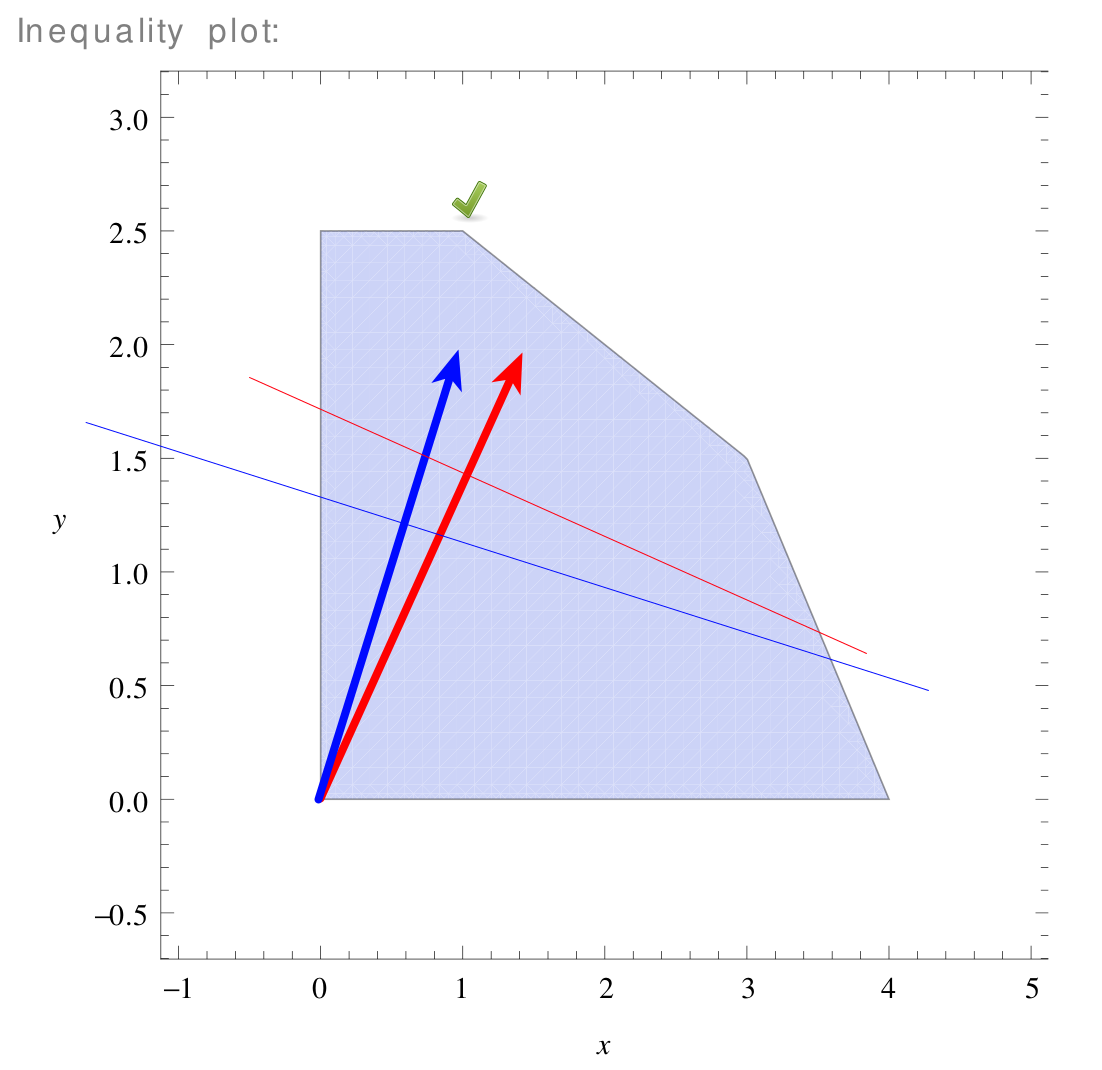
\includegraphics[width=8cm]{inequalplot.png}
\end{center}

\subsection{Linear Optimization}

\begin{enumerate}[label={\alph*)}]
  \item For $c^T = (-1, -1)$ we have to maximize $-x_1-x_2$, i.e. minimize
  $x_1+x_2$.\\
  In the feasible region, this is the case for $(x_1, x_2) = (0, 0)$.
  \item For $c^T = (0, -1)$ we have to maximize $-x_2$, i.e. minimize
  $x_2$.\\ 
  In the feasible region, this is the case for $(x_1, x_2) = (\lambda, 0)$,
  $\lambda \in [0, 1]$.
  \item For $c^T = (-1, 0)$ we have to maximize $-x_1$, i.e. minimize
  $x_1$.\\ 
  In the feasible region, this is the case for $(x_1, x_2) = (0, \lambda)$,
  $\lambda \in [0, \infty [$.
  \item For $c^T = (1, 1)$ we have to maximize $x_1+x_2$.\\
  Since e.g. the half-line $x_1-x_2=0$, $x_1, x_2 \geq 0$ lies in the feasible
  region, and as the target function increases strictly along this half-line,
  there is no optimal solution.
\end{enumerate} 
If the following constraint is added, the problem becomes infeasible:
\[
x_1-x_2 \geq 2.
\]

\subsection{Profit Optimization}

The linear program contains six inequalities:
\[ \text{max} \{
\left( \begin{array}{cc} 20 & 25 \end{array}\right)  \cdot \left( \begin{array}{c} A \\ B \end{array}\right) 
 \quad | \quad
\left( \begin{array}{cc} 1 & 0\\ -1 & 0\\ 0 & 1 \\ 0 & -1 \\ 1 & -2 \\ 1 & 2 \end{array}\right) 
\cdot
\left( \begin{array}{c} A \\ B \end{array}\right) 
\leq
\left( \begin{array}{c} 60\\ 0\\ 50 \\ 0 \\ 0 \\ 120 \end{array}\right) 
\} \]

Again, we solve it graphically, leading to the optimal solution of \$1950 profit per day.
It is reached with a daily production of $A=60$ and $B=30$ refrigerator units.

\begin{center}
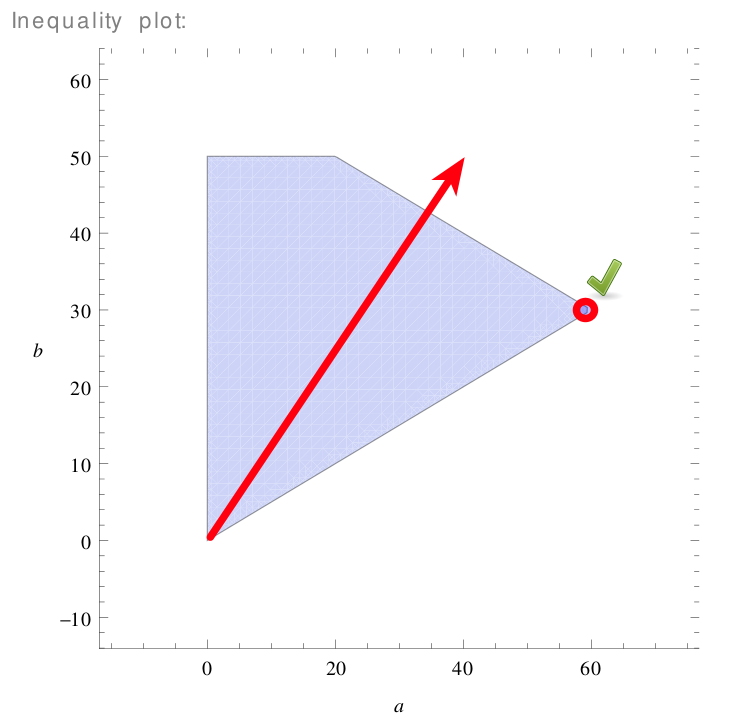
\includegraphics[width=8cm]{inequalplot4.png}
\end{center}
\end{document}
